%%%%%%%%%%%%%%%%%%%%%%%%%%%%%%%%%%%%%%%%%%%%%%%%
%%%%%%%%%%%%%Przykładowy dokument%%%%%%%%%%%%%%%
%%%%%%%%%%Wraz z klasą pracadyp.cls%%%%%%%%%%%%%
%%daje w ShareLatex w pełni czytleny plik .pdf%%
%%%%dla Otwartego Systemu Antyplagiatowego%%%%%% 
%%%%%%%WMP.SNŚ UKSW, Marek A. Kowalski%%%%%%%%%%
%%%%%%%%%%%%%%%%%%%%%%%%%%%%%%%%%%%%%%%%%%%%%%%%
\documentclass[licencjacka]{pracadypl}
%
%% ważne definicje %%
%\usepackage{tgtermes}
\usepackage[T1]{fontenc}
\usepackage{polski}
\usepackage[utf8]{inputenc}
\usepackage{hyperref}
\hypersetup{
	colorlinks,
	citecolor=black,
	filecolor=black,
	linkcolor=black,
	urlcolor=black
}
\input glyphtounicode
\pdfgentounicode=1
\usepackage{amssymb, amsthm,amsmath, tikz, indentfirst}
\hyphenation{for-singiem}
\bibliographystyle{plain}
\usepackage{wrapfig}
%\usepackage{showkeys}
\newtheorem{tw}{Twierdzenie}[chapter]
\newtheorem{np}[tw]{Przykład}
\newtheorem{obs}[tw]{Obserwacja}
\newtheorem{fakt}[tw]{Fakt}
\newtheorem{wn}[tw]{Wniosek}
\theoremstyle{definition}
\newtheorem{de}{Definicja}

\DeclareMathOperator{\spacja}{\hspace{0,1cm}}
\newcommand{\linia}{\rule{\linewidth}{0.4mm}}

\usepackage{float}

\def\uczelnia{{Uniwersytet Kardynała Stefana Wyszyńskiego w~Warszawie}\\
	Wydział Matematyczno-Przyrodniczy \\ Szkoła Nauk Ścisłych}
\def\mgr{magisterska}
\def\lic{licencjacka}
\def\inz{inżynierska}
\def\sk{Słowa kluczowe}
\def\dz{Dziedzina Socrates-Erasmus}
\def\et{English title}
\def\kt{Klasyfikacja tematyczna}
\author{Jacek Giedronowicz}
\nralbumu{95175}
\title{Rekomendacja stron www z silnikiem Apache Lucene }
\kierunek{Informatyka}
\zakres{Machine Learning}
% Praca wykonana pod kierunkiem:
% (Podając w dopełniaczu tytuł stopień imię i nazwisko opiekuna pracy
% trzeba pamiętać, że w tym przypadku prawidłową formą skrótu słowa doktor 
% jest dr w odniesieniu do kobiet i dr. w odniesieniu do mężczyzn. Możemy więc
% przykładowo zapisać, że praca została wykonana pod kierunkiem 
% prof. dr hab. Ewy Rak i prof. dr. hab. Adama Raka. Pominięcie kropki po 
% drugim "dr" byłoby błędem.
\opiekun{dr. Roberta Kłopotka}
% miesiąc i rok:
\date{Lipiec 2020}
%Słowa kluczowe:
\keywords{aplkacja webowa, wyszukiwarka, Apache Lucene}
%Podać dziedzinę pracy wg klasyfikacji Socrates-Erasmus:
\dziedzina{ 
	%11.1 Matematyka
	11.3 Informatyka 
	%13.3 Chemia
	%% pełny wykaz jest w pliku 
	%% http://www.mish.uw.edu.pl/pliki/kody_erazmus.pdf
}
%Klasyfikacja tematyczna według AMS (matematyka) lub ACM (informatyka) ...
\klasyfikacja{Machine Learning}
\tytulang{Website recommendation using the Apache Lucene engine}
%% koniec ważnych definicji %%
%
%%% autorskie definicje %%%
%%% koniec autorskich definicji %%%
%

\begin{document}
\maketitle
\tableofcontents
\thispagestyle{empty}

\chapter{Wprowadzenie}

%\linia
%\begin{itemize}
%	\item ok 1-2 str
%	\item ogólne zagadnienie jak jest stosowane w praktyce (do przewidywania)
%	\item opis, że klasyfikacja jest trudna, używa się wielu metod, że jednym z podejść jest komitet klasyfikatorów, aby poprawić skuteczność
%	\item cel pracy, hipotez badawczych
%	\item krótki opis co jest w danym rozdziale
%\end{itemize}
%	
%
%\linia

\chapter{Stan rynku}
%
%\linia
%\begin{itemize}
%	\item przede wszystkim zdefiniowanie problemu biznesowego i jego uzasadnienie.
%	\item Jakie są wyszukiwarki?
%	\item Jakie mają opcje?
%	\item strony spamerskie (zaburzają ranking)
%	\item hint: zobacz prace lic o serwisie otomoto
%\end{itemize}
%
%\linia

Na rynku istnieje wiele wyszukiwarek internetowych, lecz mało kto potrafi wymienić więcej niż pięć.
Internet zdominowała firma Google. Nawet takie znane wyszukiwarki jak Bing od Microsoft'u czy Yahoo mają zaledwie kilka procent udziału, który przedstawia się następująco:
\begin{itemize}
	\item Google - 93,37\%
	\item Bing - 3,61\%
	\item Yahoo - 1,75\%
	\item DuckDuckGo - 0,29\%
	\item Interia Katalog - 0,14\%
\end{itemize}
\begin{figure}[H]
	\centering
	\includegraphics[width=1\linewidth]{"img/popularnosc wyszukiwarek w polsce"}
	\caption{Popularność wyszukiwarek w Polsce}
	\label{fig:popularnosc-wyszukiwarek-w-polsce}
	Źródło: gs.statcounter.com – styczeń 2020
\end{figure}


W Polsce, z powodu trudności w przetwarzaniu naszego języka przez zagraniczne systemy, były próby stworzenia wyszukiwarek dedykowane dla polaków. Systemy z algorytmami rozpoznawania odmian słów w języku polskim. Największe powodzenie miała witryna szukacz.pl, która funkcjonowała przez 10 lat od 2001 do 2011 roku. Jak możemy przeczytać na stronie http://szukacz.pl/wiecej\_o\_szukaczu.html \cite{szukacz}: 

\begin{quote}
	"W szczycie swojego rozwoju, pod koniec 2007 roku, odpowiadał ze 115 milionów dokumentów w języku polskim pochodzących z miliona witryn (kolekcja „Polska”). Do połowy 2007 roku odpowiadał także z 45 milionów wyselekcjonowanych dokumentów w języku angielskim pochodzących z 2 milionów witryn (kolekcja „Świat”; tylko 4 procent pytań było skierowane do tej kolekcji)."
\end{quote}

Mimo sporej bazy dokumentów oraz przyzwoitym budżecie, również i ta witryna musiała się poddać międzynarodowemu gigantowi jakim jest Google. 
Stąd też wybrałem witrynę google.pl jako wzór, do którego będę się odnosił przy implementacji własnego systemu.
W dalszej części opiszę najważniejsze funkcjonalności witryny Google i porównam z Bing.

\section{Wyszukiwarka}
\begin{figure}[!htb]
	\minipage{0.49\textwidth}
	
\includegraphics[width=\linewidth]{img/google.jpg}
	\caption{Główna strona wyszukiwarki google}\label{google}
	\endminipage\hfill 
	\minipage{0.49\textwidth}
	
\includegraphics[width=\linewidth]{img/bing}
	\caption{Główna strona wyszukiwarki bing}\label{bing}
	\endminipage
\end{figure}

Na rysunkach~\ref{google} i \ref{bing} przedstawiono główne strony wyszukiwarek Google i bing. Jak widać obie strony są minimalistyczne i intuicyjne. Witryny oferują również możliwość jej spersonalizowania przez bogatą bazę skórek, co zostało przedstawione na rysunkach~\ref{google-background} i \ref{bing-background}

\begin{figure}[!htb]
	\minipage{0.49\textwidth}
	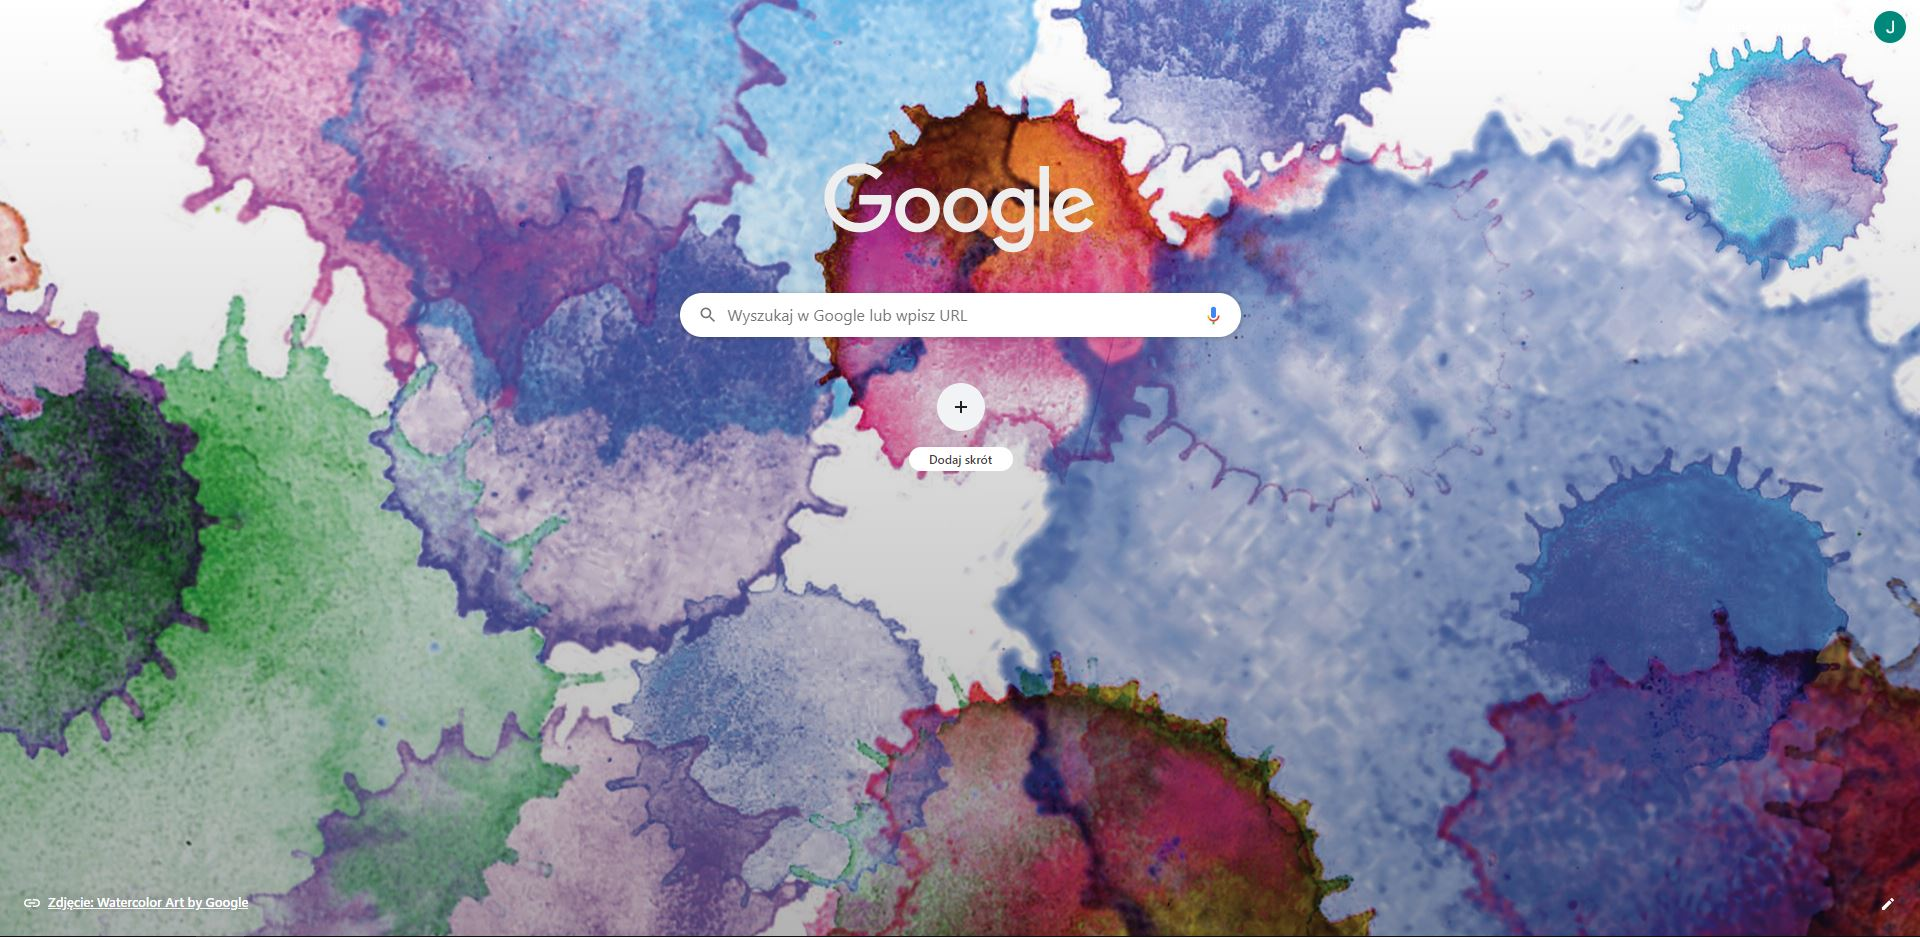
\includegraphics[width=\linewidth]{img/google-background}
	\caption{Główna strona wyszukiwarki Google ze skórką} \label{google-background}
	\endminipage\hfill 
	\minipage{0.49\textwidth}
	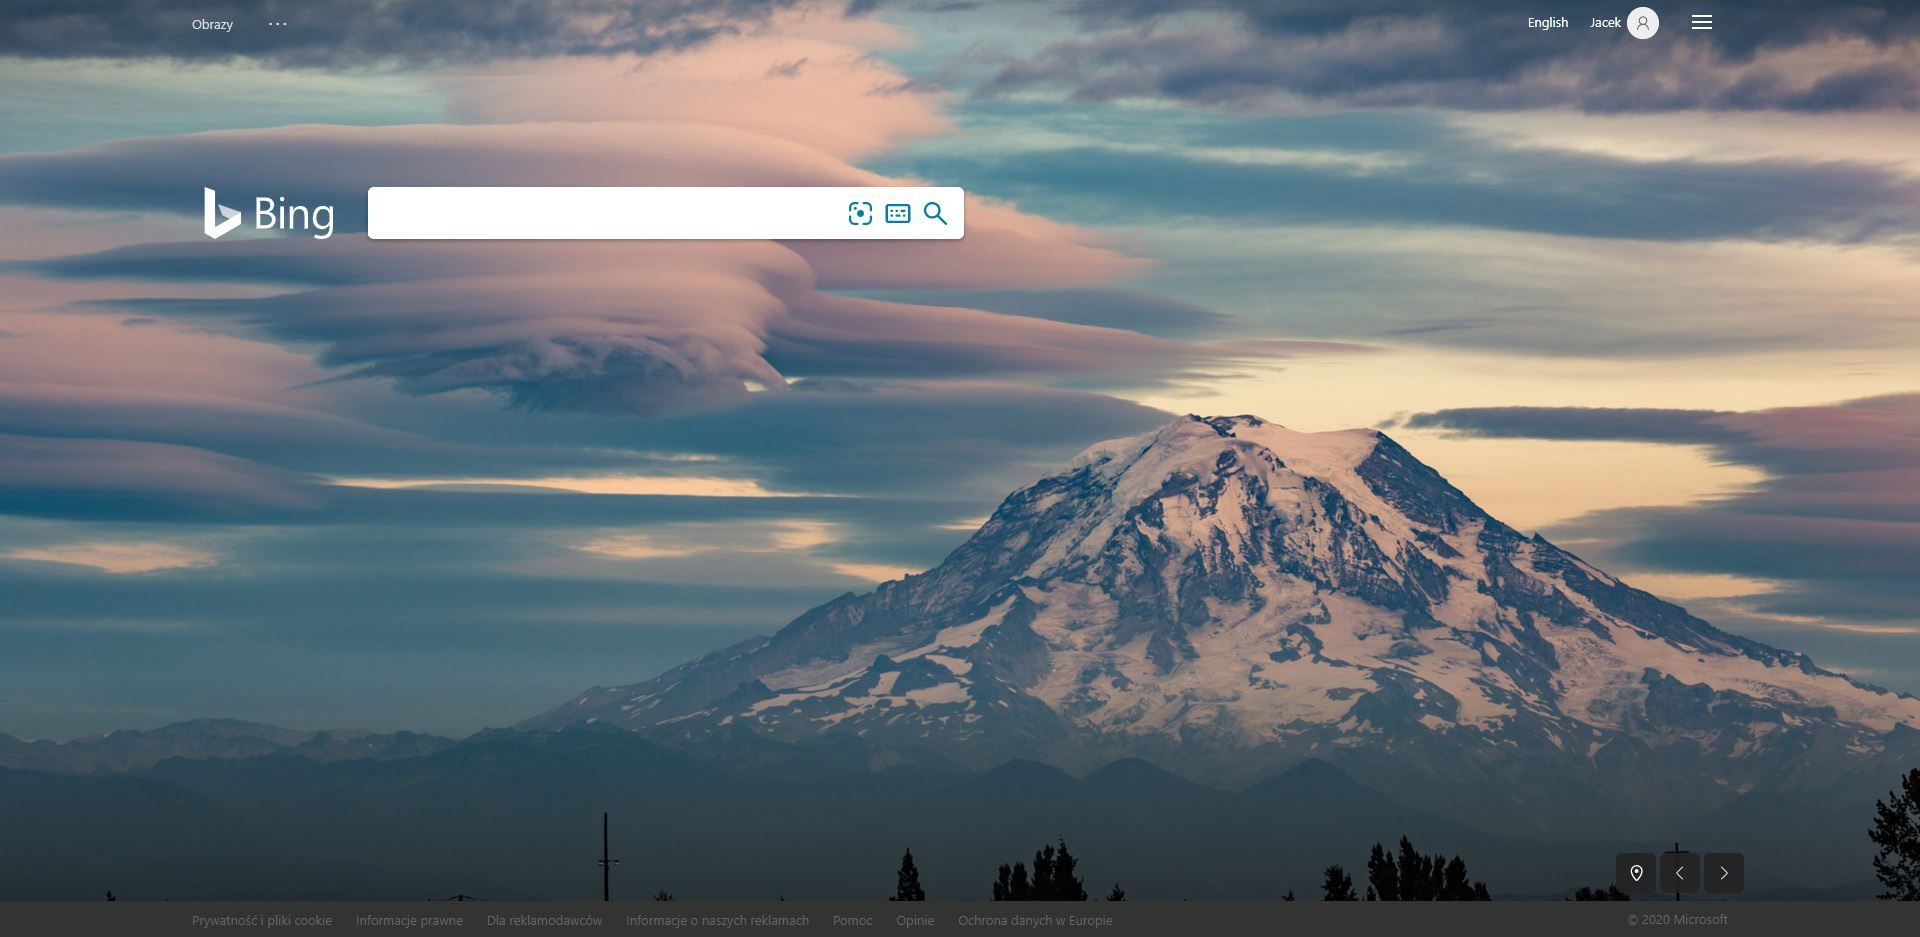
\includegraphics[width=\linewidth]{img/bing-background}
	\caption{Główna strona wyszukiwarki Bing ze skórką} \label{bing-background}
	\endminipage
\end{figure}

\section{Wyszukiwanie}

Po wpisaniu frazy, którą chcemy wyszukać obie wyszukiwarki wypiszą nam listę od kilkudziesięciu tysięcy do nawet kilkuset milionów rekomendowanych stron dla tego hasła.

Dla przykładu dla frazy ,,kobiety biznesu'' Google znalazło 125~000~000 wyników kiedy Bing zaledwie  341~000. Dominacja wyszukiwarki Google wśród użytkowników oraz zdecydowanie większa pula zaindeksowanych stron może być powodem dlaczego współcześni deweloperzy przygotowują swoje strony głównie pod pozycjonowanie wyszukiwarki Google.

\begin{figure}[!htb]
	\minipage{0.49\textwidth}
	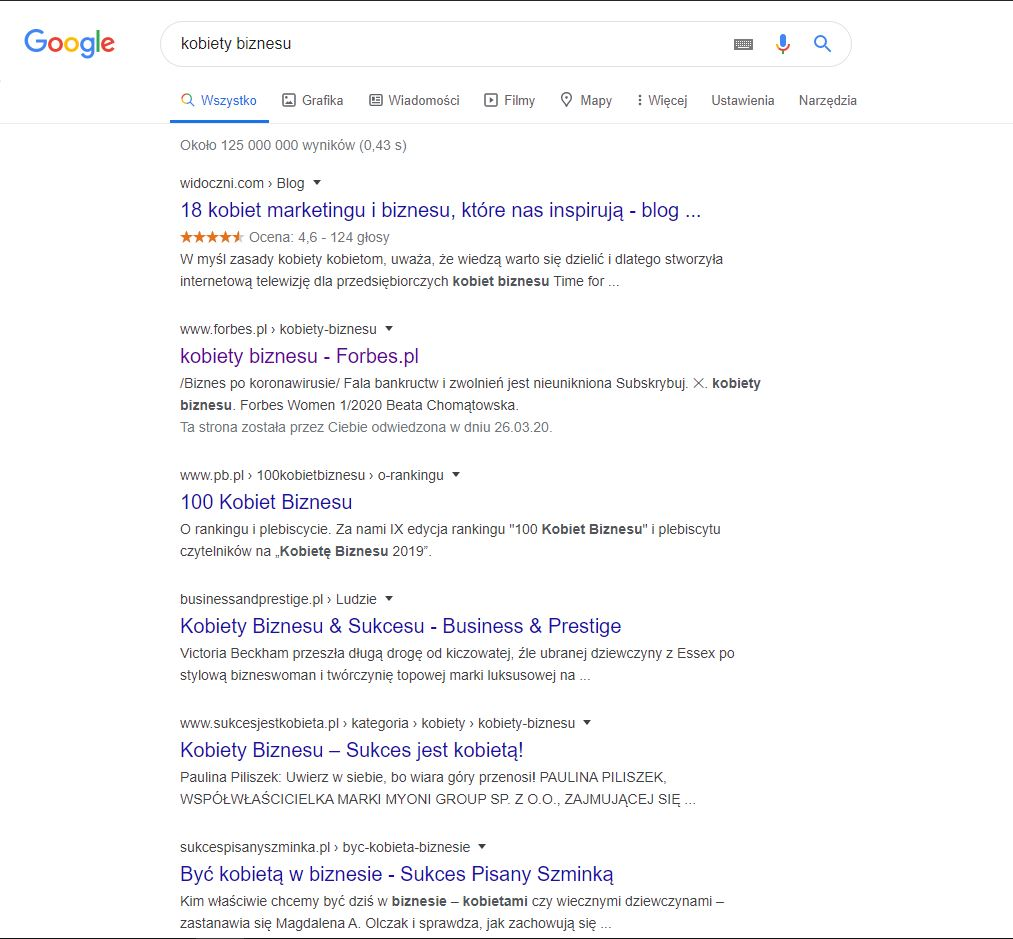
\includegraphics[width=\linewidth]{img/google-query}
	\caption{Lista rekomendowanych przez Google stron dla hasła: kobiety biznesu} \label{google-query}
	\endminipage\hfill 
	\minipage{0.49\textwidth}
	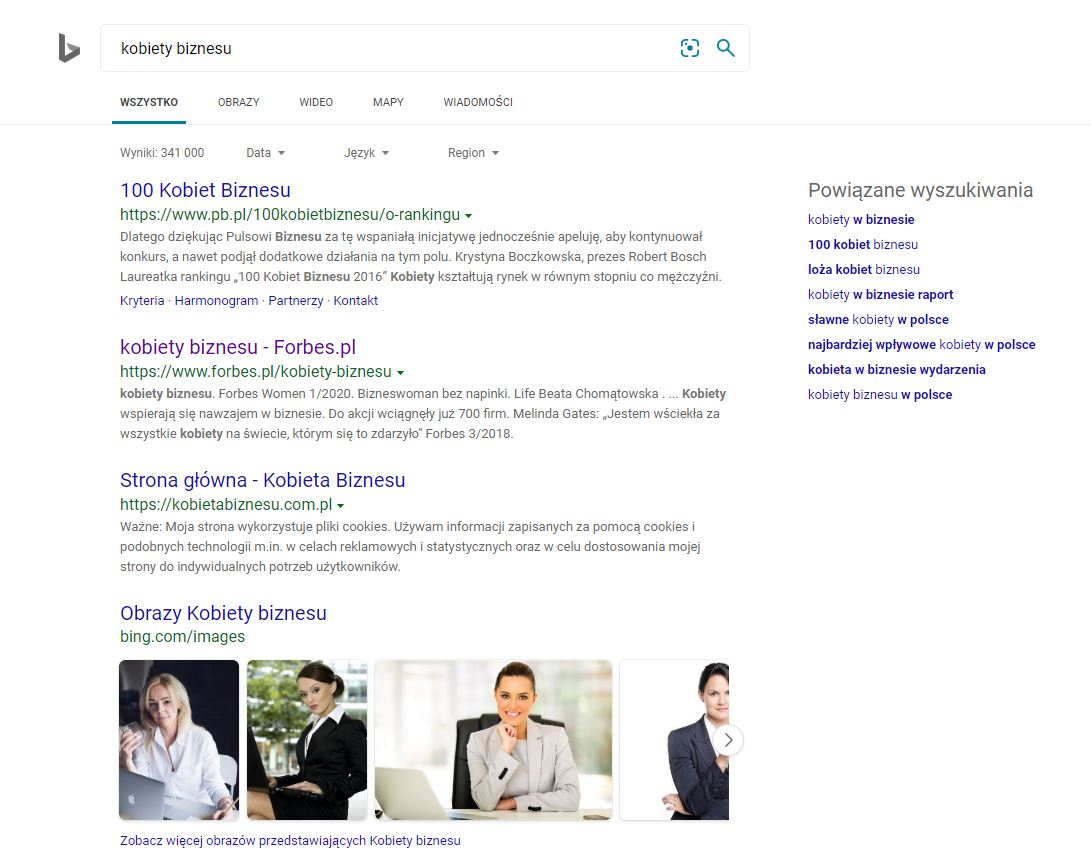
\includegraphics[width=\linewidth]{img/bing-query}
	\caption{Lista rekomendowanych przez Bing stron dla hasła: kobiety biznesu} \label{bing-query}
	\endminipage
\end{figure}


Każda z wyświetlanych pozycji przekazuje nam podstawowe informacje takie jak:
\begin{itemize}
	\item tytuł strony (zaznaczony kolorem zielonym)
	\item link do strony (zaznaczony kolorem fioletowym)
	\item skrót zawartości strony (zaznaczony kolorem brązowym)
\end{itemize}


\newpage

\begin{figure}[!htb]
	\minipage{0.49\textwidth}
	
\includegraphics[width=\linewidth]{img/google-responseBody}
	\caption{Wyświetlana pozycja w liście wyników google} \label{google-responseBody}
	\endminipage\hfill 
	\minipage{0.49\textwidth}
	
\includegraphics[width=\linewidth]{img/bing-responseBody}
	\caption{Wyświetlana pozycja w liście wyników bing} \label{bing-responseBody}
	\endminipage
\end{figure}

\begin{figure}[!htb]
	\minipage{0.49\textwidth}
	
\includegraphics[width=\linewidth]{img/google-responseBodyPlus}
	\caption{Wyświetlana pozycja w liście wyników Google z zaznaczonymi obszarami} \label{google-responseBodyPlus}
	\endminipage\hfill 
	\minipage{0.49\textwidth}
	
\includegraphics[width=\linewidth]{img/bing-responseBodyPlus}
	\caption{Wyświetlana pozycja w liście wyników Bing z zaznaczonymi obszarami} \label{bing-responseBodyPlus}
	\endminipage
\end{figure}

Oprócz podstawowego wyszukiwania linków do stron, mamy możliwość wybrania kategorii przedstawione na rysunkach~\ref{google-category} i \ref{bing-category} takich jak:
\begin{itemize}
	\item grafika
	\item wiadomości
	\item filmy
\end{itemize}

\begin{figure}[!htb]
	\minipage{0.49\textwidth}
	
\includegraphics[width=\linewidth]{img/google-category}
	\caption{Kategorie i filtry wyszukiwania Google} \label{google-category}
	\endminipage\hfill 
	\minipage{0.49\textwidth}
	
\includegraphics[width=\linewidth]{img/bing-category}
	\caption{Kategorie i filtry wyszukiwania Bing} \label{bing-category}
	\endminipage
\end{figure}

Ponadto wyszukiwarki dają nam możliwość intuicyjnego filtrowania wyników. W tym punkcie wyszukiwarki nieznacznie się różnią, gdyż Bing oferuje takie parametry jak: data, język, region. Natomiast Google: data, język i możliwość pokazania dokładnych wyników zawężając o wyniki fraz bliskoznacznych. 

\section{Podstawowe operatory}
Aby podnieść jakość i zawęzić pole poszukiwań pożądanych informacji przez użytkownika, Google zaimplementowało tak zwane operatory. 
Operatory definiują zakres poszukiwań poprzez słowa i znaki kluczowe:
\begin{itemize}
	\item \emph{" "} - wpisując wyrażenie w cudzysłów wymusza ścisłe dopasowanie. 
	Przykład: fraza \emph{"Steave Jobs"} wpisana z cudzysłowem wymusza aby w wyniku były dokładnie te dwa słowa obok siebie.
	
	\item \emph{OR} - operator logiczny pozwalający z zapytanie \emph{Steave OR Jobs} wyszukać wyniki zawierające frazę \emph{Steave} lub \emph{Jobs} lub oba.
	Operator można zastąpić znakiem $|$.
	
	\item \emph{AND} - domyślny operator logiczny, wyświetlający tylko te wyniki, które zawierają frazę \emph{Steave} i \emph{Jobs}. Operator jest domyślny więc przydatny jest tylko w połączeniu z innymi operatorami.
	
	\item $-$ - operator wykluczający. W przykładzie \emph{jaguar speed -car} wynikiem będą strony powiązane z frazą \emph{jaguar speed} ale niezawierające \emph{car}. Zatem chodziło nam o znalezienie prędkości jaguara będącego zwierzęciem a nie samochodem.
	
	\item \emph{..} - operator zakresu liczb. Przykład: \emph{podatki 2010..1015} da nam wynik wyszukiwania związanymi z podatkami miedzy 2010 a 2015 rokiem.
	
	\item \emph{( )} - operator grupowania fraz z innymi operatorami. 
	Przykład: \emph{(iPad OR iPhone)apple}. Operator \emph{AND} jest domyślny więc nie jest obowiązkowy.
	
	\item \emph{define:} - operator wyszukuje definicje szukanej frazy.
	
	\item \emph{filetype:} lub \emph{ext:} - operator określający rodzaj pliku będący wynikiem wyszukiwania takie, jak pdf, docx, txt, ppt.
	Przykład: \emph{Steve Jobs ext:pdf} - wyświetli tylko pliki pdf związane ze Steve'em Jobs'em. 
	
	\item \emph{site:} - ogranicza wyniki wyszukiwania tylko do jednej strony lub domeny.
	Przykład: \emph{wniosek site:.gov.pl} wyszuka informacje o wnioskach tylko na stronach rządowych kończących się na \emph{.gov.pl}.

	\item \emph{inurl:} - operator przeszukuje podaną frazę tylko w adresie url strony.
		
	\item \emph{intitle:} - operator przeszukuje podaną frazę tylko w tytule strony.
	
	\item \emph{intext:} - operator przeszukuje podaną frazę tylko w treści strony. Pominie strony zawierające frazę w tytule czy adresie url.
	
\end{itemize}

Google zawiera znacznie więcej operatorów. Niektóre z nich wymienione są na stronie sites.google.com \cite{operatory-google}

\chapter{Rekomendacja stron www}
Cały algorytm możemy podzielić na dwa etapy: indeksowanie i wyszukiwanie.
Użytkownik oczekuje od aplikacji szybkiego i trafnego wyszukiwania jednak, aby tak się stało trzeba najpierw zebrać wszystkie dane i nadać im specjalną strukturę dzięki której będziemy mogli szybko znaleźć interesującą nas informacje. To właśnie nazywamy procesem indeksowania.


\section{Proces indeksowania}

\subsection{Document}

\begin{wrapfigure}{R}{0.4\textwidth}
	\centering
	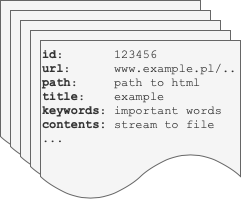
\includegraphics[width=0.3\textwidth]{img/documents.png}
	\caption{Struktura dokumentu}
\end{wrapfigure}
Dokument reprezentuje stronę internetową. Jest główną jednostką indeksowania i wyszukiwania.
Technicznie jest zbiorem (kontener typu \texttt{Set}) zawierający pola (\texttt{field}) złożone z klucza i wartości.
Dzięki temu możemy zapisać w ustrukturyzowany sposób najważniejsze dla nas informacje, po których później będziemy wyszukiwać.
Do wyszukiwania stron www przydatne będą takie pola jak :
\begin{itemize}
	\item \texttt{id} - unikalny identyfikator dokumentu
	\item \texttt{url} - adres url strony
	\item \texttt{path} - ścieżka do kodu html na dysku twardym
	\item \texttt{title} - tytuł strony
	\item \texttt{keywords} - słowa kluczowe z meta znacznika \texttt{<meta name="keywords">}
	\item \texttt{description} - opis strony z mata znacznika\texttt{<meta name="description">}
	\item \texttt{headers} - nagłówki ze znaczników \texttt{<h1>} do \texttt{<h6>} 
	\item \texttt{emphasize} - wyróżnione słowa za pomocą znaczników takich jak \texttt{<em>,<b>,<strong><i>,<mark>}
	\item \texttt{images} - informacje o obrazach dostępnych na stronie
\end{itemize}


\subsection{Struktura indeksu}

Index jest pojedynczym katalogiem na dysku struktury drzewiastej \cite{lucene-article}. Składa się z segmentów (\texttt{segment}), dokumentów (\texttt{document}), pól (\texttt{field}), wyrażeń (\texttt{term}).
Segmenty można traktować jak pod-indeks jednakże nie stanowią one niezależnych indeksów. 
Liczba tworzących je plików zależy od liczby pól zawartych w indeksie.
Wszystkie pliki należące do tego samego segmentu mają taki sam prefiks ale różnią się sufiksem. 


\begin{figure}[H]
	\centering
	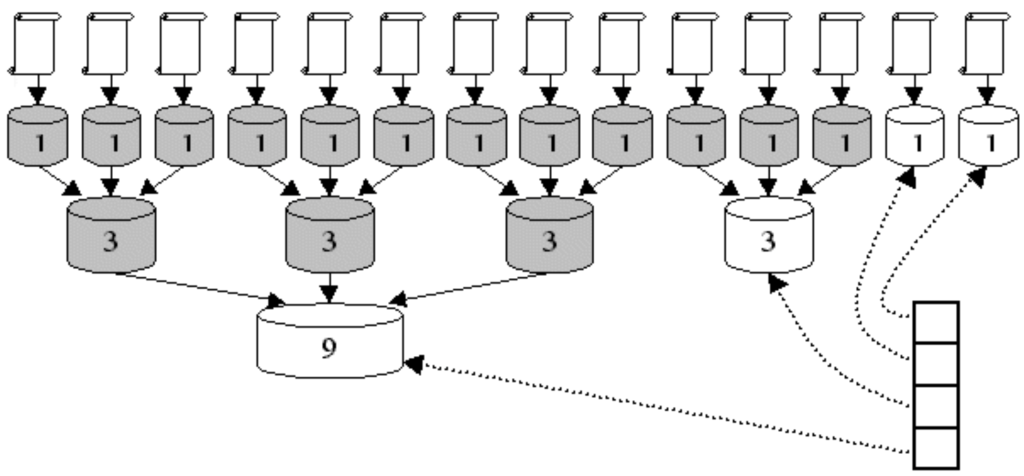
\includegraphics[width=1\linewidth]{img/segments.png}
	\caption{Struktura indeksu \cite{alg-on-cloud}}
\end{figure}

Wyrażenia zapisane w dokumencie (\texttt{term}) są analizowane i zapisywane w specjalnej strukturze zwanej inverted index. Polega ona na przedstawieniu relacji \texttt{document - term} w postaci tabeli przedstawionej na rysunku \ref{inverted-index}. Możemy nie niej szybko znaleźć wyrażenie i id dokumentu, który zawiera dane wyrażenie.

\begin{figure}[H]
	\centering
	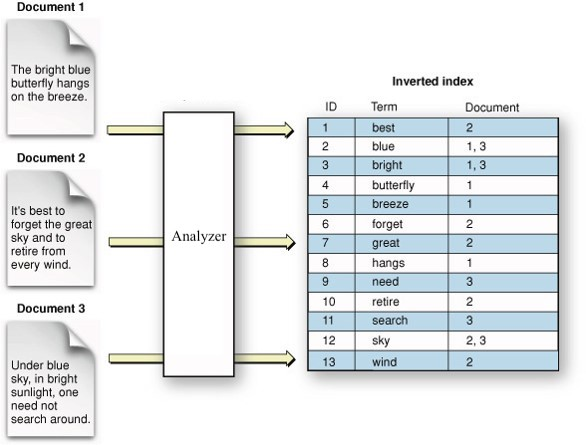
\includegraphics[width=1\linewidth]{img/inverted-index.jpg}
	\caption{Struktura indeksu}
	\label{inverted-index}
\end{figure}

Powyższy sposób pozwala nam na szybkie znalezienie interesującego nas wyrażenia - dzięki analyzerowi wyrażenia będące uosobieniem tego samego słowa, niezależnie od formy gramatycznej, zajmują jeden rekord w bazie w postaci najprostszego wyrażenia.

\subsection{Analyzer}

Analyzer jest mechanizmem analizowania tekstu i generowania tak zwanych \texttt{token}'ów - będącymi jednostkami leksykalnymi. Dzięki temu dla programu słowa "wyrazić, wyrażenia, wyrażenie" to jedno i to samo.

Dla różnych potrzeb i co ważniejsze dla różnych języków zostały stworzone różne analyzery. Przykładowo:
\begin{itemize}
		\item \texttt{WhitespaceAnalyzer}\\
	Rozdziela tekst bazując na białych znakach (spacja).
	Przykład.
	$$	\texttt{["This is an example term analysis test."]}$$
	$$\downarrow$$
	$$\texttt{["This", "is", "an", "example", "term", "analysis", "test."]}$$
		
	\item \texttt{SimpleAnalyzer}\\
	Rozdziela tekst bazując na nieliterowych znakach takich jak liczby, znaki białe czy interpunkcja i zmienia je na małe znaki.
	Przykład.
	$$	\texttt{["This is an 1example term analysis test."]}$$
	$$\downarrow$$
	$$\texttt{["this", "is", "an", "example", "term", "analysis", "test"]}$$
	
	\item \texttt{StopAnalyzer}\\
	Rozdziela tekst bazując na białych znakach. Usuwa interpunkcje oraz takie słowa jak 'a', 'an', 'the' itp
	Przykład.
	$$	\texttt{["This is an example term analysis test."]}$$
	$$\downarrow$$
	$$\texttt{["example", "term", "analysis", "test"]}$$
	
	\item \texttt{StandardAnalyzer}\\
	Standardowy analyzer obsługujący nazwy, adresy email itp. 
	Zmienia wszystkie znaki na małe oraz usuwa interpunkcje i zaimki/przedimki.
	Przykład.
	$$	\texttt{["This is an example term analysis test."]}$$
	$$\downarrow$$
	$$\texttt{["example", "term", "analysis", "test"]}$$


	\item \texttt{PolishAnalyzer}\\
	Odpowiedni analyzer dla języka polskiego. Zmienia litery na małe, usuwa interpunkcje i co najważniejsze zmienia podane wyrażenia na ich podstawową formę (o ile to możliwe bezokolicznik lub mianownika).
	Przykład.
	$$	\texttt{["To jest przykładowy test analizy wyrażenia."]}$$
	$$\downarrow$$
	$$\texttt{["przykładowy", "test", "analiza", "wyrazić"]}$$
	
\end{itemize}

W procesie wyszukiwania będziemy musieli użyć dokładnie tego samego analyzera do przygotowania zapytania.


\section{Proces wyszukiwania}

\begin{wrapfigure}{R}{0.45\textwidth}
	\centering
	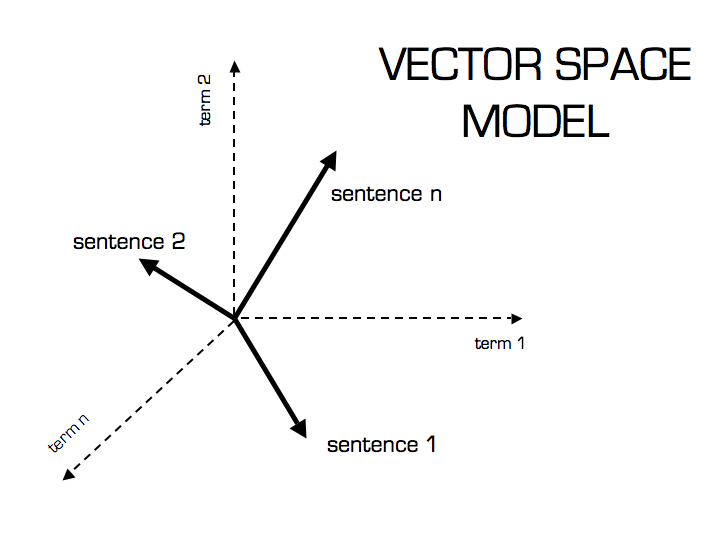
\includegraphics[width=1\linewidth]{img/vector-space.png}
	\caption{VSM}
\end{wrapfigure}

Po zaindeksowaniu wszystkich dokumentów możemy je teraz przeszukiwać.
Proces wyszukiwania przechodzi po indeksie szukając najlepszego dopasowania do naszego zapytania (\texttt{Query}), przeanalizowanego przez nasz analyzer. 
Do punktowania (\texttt{Scoring}) wykorzystywany jest model podobieństwa TF-IDF (\texttt{TF-IDF Similarity}) implementujący model przestrzeni wektorowej (\texttt{Vector Space Model - VSM} ).
W \texttt{VSM} im więcej razy dane słowo pojawia się w dokumencie w stosunku do frekwencji we wszystkich dokumentach tym wyżej punktowany jest.

\subsection{TF-IDF Similarity}
Podobieństwo TF-IDF (term frequency – inverse document frequency) \cite{similarity-documentation} jest metodą obliczania wagi słów w oparciu o liczbę ich wystąpień. Mierzone jest w modelu VSM, w którym zarówno dokumenty jak i zapytania reprezentowane są jako wektory ważone w przestrzeni wielowymiarowej.

Załóżmy, że $t$ oznacza term oraz $d$ dokument.
Wartość podobieństwa TF-IDF termu $t$ dla dokumentem $d$ oblicza się ze wzoru:
\[
	tfidf(t) = tf(t,d) \times idf(t)
\]
gdzie $tf(t,d)$ nazywamy frekwencją termu (\texttt{term frequency}) i wyrażamy wzorem
\[
	tf(t,d) = 
	\frac{n_{t,d}}{\sum_{k} n_{k,d}}
\]
gdzie $n_{t,d}$ jest liczbą wystąpień termu $t$ w dokumencie $d$.

$idf(t)$ nazywamy odwróconą frekwencją dokumentów (\texttt{inverse document frequency}) wyrażona wzorem
\[
	idf(t) = \log 
	\frac 
	{ |D| }
	{ 1 + |\{ d \colon t \in d \}| }
\]
gdzie $|D|$ jest liczbą dokumentów a $|\{ d \colon t \in d \}|$ jest liczbą dokumentów zawierających dany term. Dodając jedynkę tj $1 + |\{ d \colon t \in d \}|$ zabezpieczamy się przed dzieleniem przez $0$. 


Dla lepszej jakości wyszukiwań i bezpieczeństwa,  dobra wyszukiwarka nie polega tylko na podobieństwie.
Bierze również pod uwagę czy strona znajduje się w cenionej witrynie, czy witryna jest niskiej jakości albo nawet spamuje. Takie witryny powinny być odnotowane na specjalnej liście spamerskiej a wyszukiwarka nie powinna rekomendować żadnych stron z danej witryny.

Za to punktacje wysokiej jakości stron może podnieść tak zwany PageRank.

\newpage
\subsection{PageRank}
%\begin{wrapfigure}{R}{0.45\textwidth}
%	\centering
%	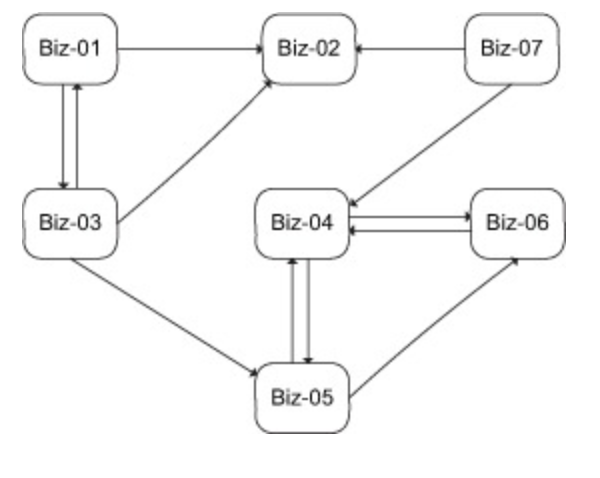
\includegraphics[width=1\linewidth]{img/pagerank-graph.png}
%	\caption{Przykład grafu skierowanego }
%\end{wrapfigure}

Algorytm opracowany przez założyciela Google - Larry'ego Page'a i Sergey'a Brin'a \cite{google-how-search-works}. 
Kluczową ideą jest rozważanie hiperłączy z jednej strony internetowej na drugą.
Im więcej linków prowadzi do danej strony, tym ważniejsze ma znaczenie. 
Innymi słowy, jeśli strona internetowa jest wskazywana przez inne, ważne strony, to jest to również ważna strona.

Sieć połączeń stron hiperłączami tworzy graf skierowany.
\begin{de}
	$G := (V,E)$ nazywamy grafem skierowanym. 
	Zbiór $V \neq \emptyset$ jest zbiorem elementów zwanych wierzchołkami.
	Zbiór $E \subseteq 
	\big\{
		\{ u,v \} \colon u,v \in V
	 \big\}$
	 nazywamy zbiorem krawędzi skierowanych z wierzchołka $u \in V$ do wierzchołka $v \in V$
	 oraz $\deg(u)$ liczbą krawędzi wychodzących z wierzchołka $u \in V$.
\end{de}

\begin{de}
	Niech $u$ będzie stroną internetową. 
	Wtedy $F_u$ będzie zbiorem stron, na które $u$ wskazuje oraz $B_u$ zbiorem stron, które wskazują na $u$.
	\begin{figure}[H]
		\centering
		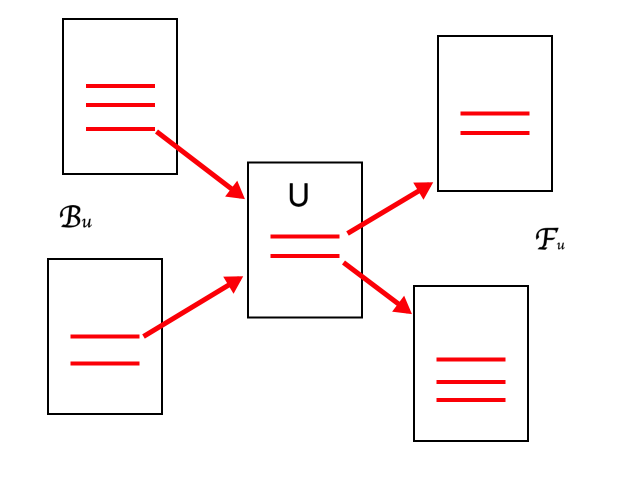
\includegraphics[width=0.4\linewidth]{img/pagerank-link.png}
		\caption{Zbiory $F_u$ i $B_u$}
	\end{figure}
	
	PageRank $R$ strony $u$ jest zdefiniowany następująco:
	\[
	R(u) = 
	\frac{1-d}{N} +
	d \cdot 
	\sum\limits_{i=1}^{|B_u|}
	\frac{R(B_i)}
	{\deg(B_i)}
	\]
	gdzie $N$ jest liczbą dokumentów oraz $d$ jest parametrem wybranym eksperymentalnie ( zwykle $d=0.85$) nazywany współczynnikiem tłumienia (\textit{Damping factor}).
	Suma wartości wektora $R = \big[ R_{u_1}, R_{u_2}, \dots R_{u_N} \big]$ jest równa $1$, 
	tj. $\sum_{i=0}^{N} R_{u_i} = 1$.
	
\end{de}
\begin{figure}[H]
	\centering
	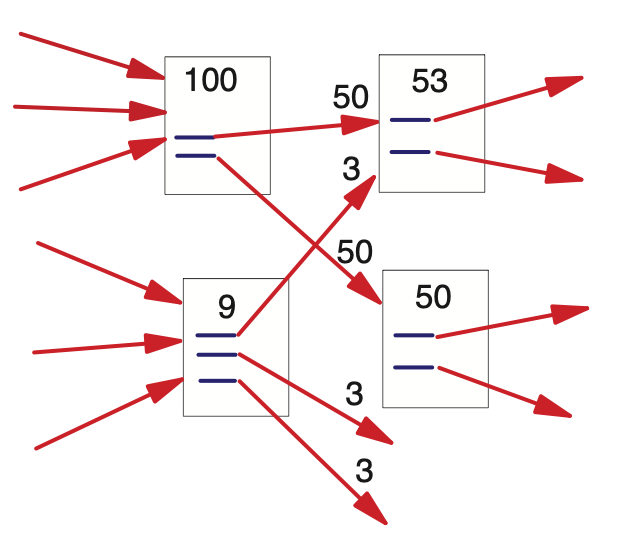
\includegraphics[width=0.4\linewidth]{img/pagerank-link2.png}
	\caption{Przykład uproszczonego PageRank}
\end{figure}

Powstaje problem typu \textit{Cold Start} - do obliczeń PageRank danej strony potrzebujemy PageRanku stron do niej podlinkowanych, gdzie początkowo żadna ze stron nie posiada wyliczonego rankingu.

Wartości te można wyliczyć w sposób iteracyjny.
Przyjmijmy początkowy rozkład prawdopodobieństwa dla czasu $t = 0$ :
\[
	R(u;0) = \frac{1}{N}
\]
Następnie nasz wzór z czasem $t$: 
	\[
		R(u ; t + 1) = 
		\frac{1-d}{N} +
		d \cdot 
		\sum\limits_{b_i \in B_u}
		\frac{R(b_i ; t)}
		{\deg(b_i)}
\]
jest obliczany iteracyjnie dla każdej strony $u$ należącej do grafu,
gdzie $R(p ; t)$ jest rankingiem strony $p$ w czasie $t$ oraz $d$ jest współczynnikiem tłumienia.
Iteracje możemy przerwać gdy wartości PageRank przestaną się zmieniać w stopni znacznym tj.
$\big| R(t+1) - R(t) \big| < \epsilon$ dla pewnego ustalonego $\epsilon > 0$.

Założyciele google'a w swoim raporcie \cite{pagerank-report} opisali, że do obliczenia PageRank'u dla 322 milinów stron wystarczyły 52 iteracje. Dla o połowę mniejszej bazy 42 iteracje, wyciągając wnioski, że współczynnik skalowania jest równy $\log N$.

\begin{figure}[H]
	\centering
	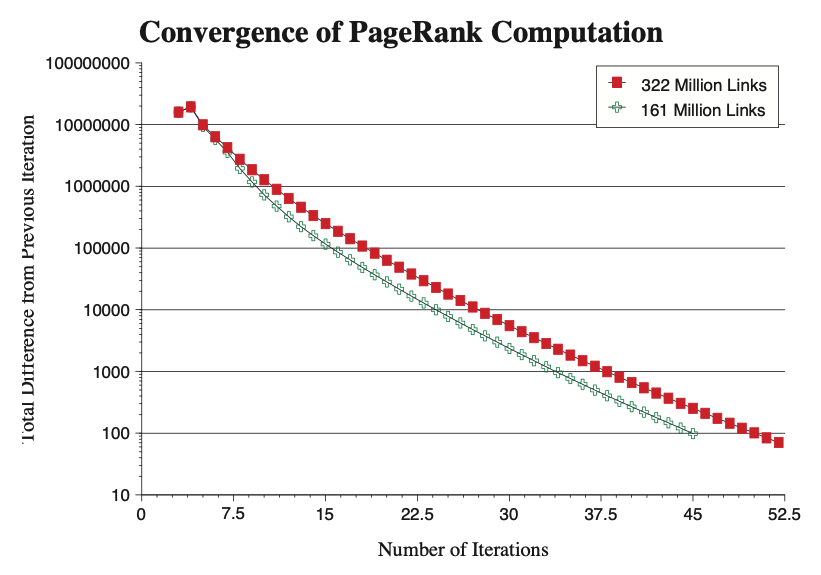
\includegraphics[width=0.6\linewidth]{img/pagerank-iteracja}
	\caption{Iteracje w obliczeniach PageRank}
\end{figure}

Macierz PageRank jest łańcuchem Markowa, gdzie z teorii Markowa, jego wartość $R(u)$ jest prawdopodobieństwem przejścia ze strony $u$ z powrotem do strony $u$ po dużej liczbie przejść w błądzeniu losowym (\textit{Random Walk}).

\begin{de}
	Łańcuchem Markowa o zbiorze stanów $V$ nazywamy ciąg zmiennych losowych $X_0, X_1,X_2, \dots$ takich, że 
	\[
	\mathbb{P} 
	\big(
	X_n = v_n \big| X_{n-1} = v_{n-1} \wedge
	\dots
	X_0 = v_0
	\big) = 
	\mathbb{P} 
	\big(
	X_n = v_n \big| X_{n-1} = v_{n-1}\big)
	\]
	Oznacza to, że prawdopodobieństwo przejścia jest niezależne od $n$.
\end{de}



\subsection{Power Method}

Dla szybszego niwelowania błędu w iteracji do obliczania PageRank wykorzystano algorytm Power Method bazujący na wartościach własnych macierzy.

Niech macierz $\mathcal{M} = \big[ \mathcal{M}_{i,j} \big]_{}$ będzie macierzą przejścia zdefiniowaną następująco:
$$\mathcal{M}_{i,j} = 
\left\{ 
\begin{array}{ll}
	\frac{1}{\deg(p_i) }	 & 	\text{jeśli strona $p_i$ jest podlinkowana do $p_j$}	\\
	0								&	\text{w p.p}
\end{array}
\right.$$

oraz PageRank $R$ będzie rozkładem prawdopodobieństwa tj. $\big|R\big| = 1$ i  $\mathbf{E}R = 1$ gdzie $\mathbf{E}$ jest macierzą jedynek.
Wtedy \textit{Power Method PageRank} jest dany wzorem: 
\[
	R = 
	\left( 
		d \mathcal{M} + 
		\frac{1 -d}{N} \mathbf{E}
	\right)
	R
\]

\subsection{Dangling Nodes Problem}

Podczas obliczania PageRank pojawia się \textit{Dangling Nodes Problem} czyli problem stron, które nie posiadają linków wychodzących. 

\begin{figure}[H]
	\centering
	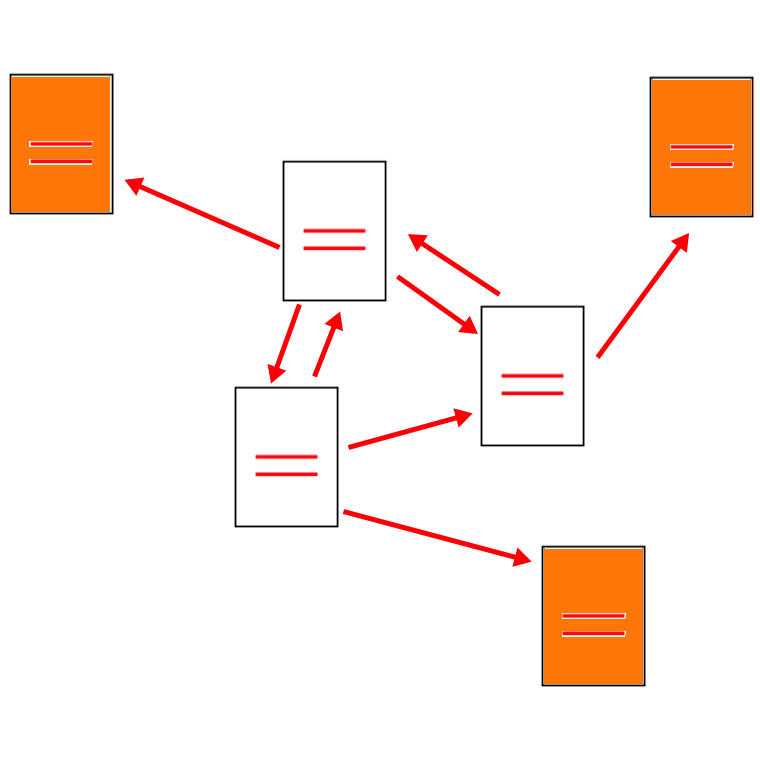
\includegraphics[width=0.4\linewidth]{img/pagerank-dangling-node}
	\caption{Przykład grafu z Dangling Nodes}
\end{figure}

Stawiają kłopotliwe pytanie dla modelu, gdzie ich wartość powinna zostać dalej dystrybuowana.
Istnieją dwa rozsądne rozwiązania:
\begin{itemize}
	\item \textbf{Usunąć na czas obliczeń}
	\begin{figure}[H]
		\centering
		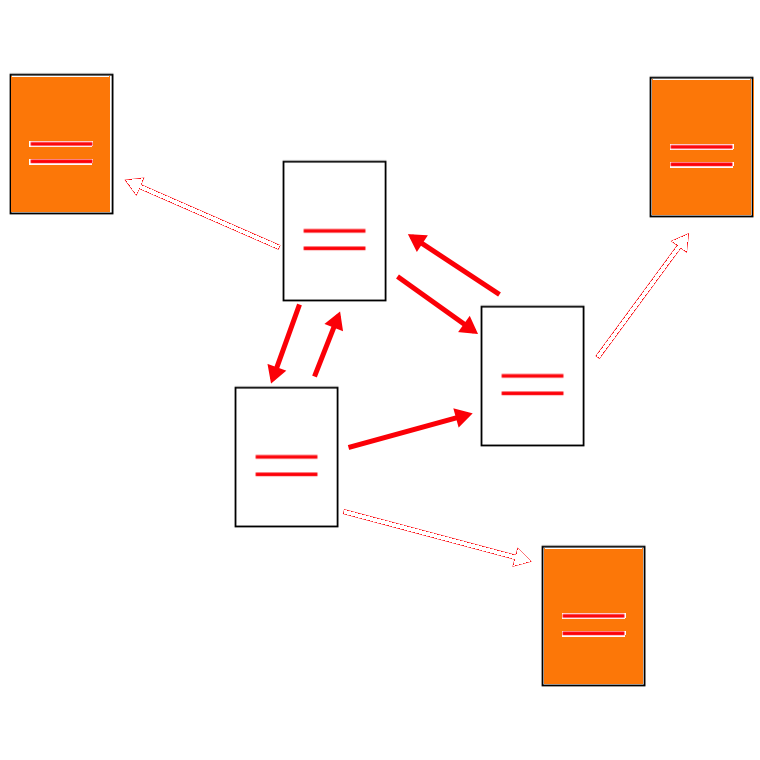
\includegraphics[width=0.4\linewidth]{img/pagerank-without-dangling-node}
		\caption{Przykład usuwania Dangling Nodes}
	\end{figure}
Skoro Dangling Nodes nie wpływa bezpośrednio na PageRank żadnej innej strony, możemy je po prostu wykluczyć z naszych obliczeń. 
Takie strony stanowią dużą część grafu stąd usunięcie ich z obliczeń może okazać się korzystne dla czasu realizacji.
	
	\item \textbf{Dodać tymczasowy wierzchołek}
		\begin{figure}[H]
		\centering
		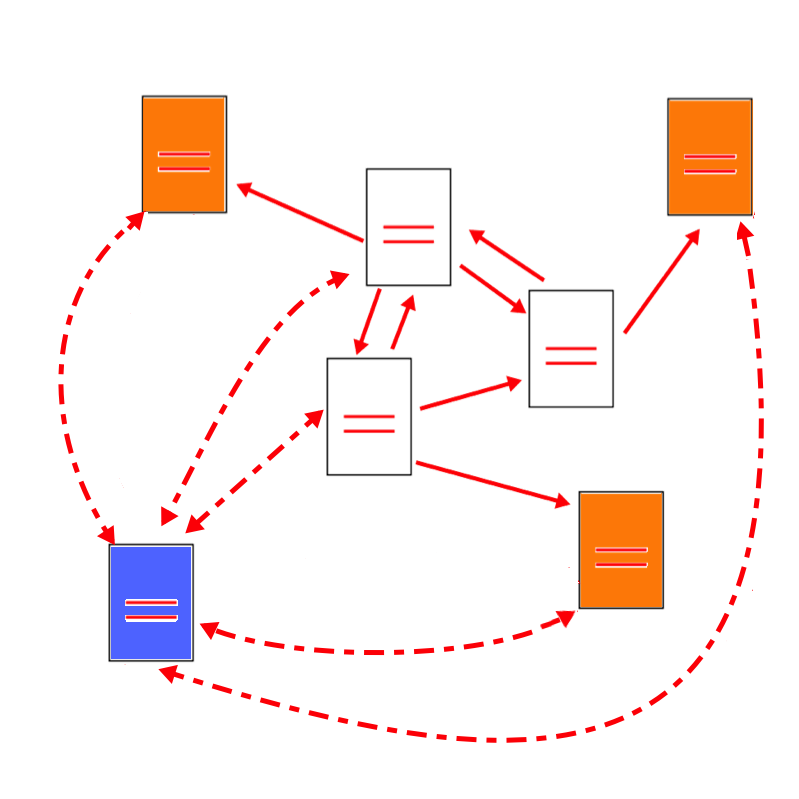
\includegraphics[width=0.4\linewidth]{img/pagerank-withextra-dangling-node}
		\caption{Przykład usuwania Dangling Nodes}
	\end{figure}
\end{itemize}
Na czas obliczeń możemy dodać tymczasowy wierzchołek, który będzie połączony dwukierunkowo ze wszystkimi wierzchołkami w grafie.
%TODOD dzieki temu... co ? jaki jest jego pagerank?

%chapter{Przedstawienie problemu i sposób jego rozwiązania}
%\linia
%\begin{itemize}
%	\item Przede wszystkim przedstawienie tego problemu, który będzie opisany w pracy
%	\item problem przedstawiony w pracy może być jednym z podproblemów ogólnego problemu biznesowego
%	\item opis metod lub algorytmów np w postaci pseudokodu lub schematów 
%	\item uzasadnienie użytych metod
%	\item testy kilku parametrów, przygotowanie danych itd.
%\end{itemize}
%
%\linia

\chapter{Funkcjonalność zaimplementowanego systemu}
%\linia
%\begin{itemize}
%	\item opis jakie funkcjonalności będzie miał system
%	\item w jaki sposób dana funkcjonalność przyczyni się do rozwiązania problemu
%\end{itemize}
%
%\linia
\section{Wyszukiwarka}
\section{Wyszukiwanie}
\section{Podstawowe operatory}


\chapter{Implementacja oraz użyte technologie}
%\linia
%\begin{itemize}
%	\item dokładnie jak zostało to wszystko implementowane
%	\item opis architektury
%	\item jaka platforma, diagram klas, jaka funkcjonalność jest w jakiej klasie/module/package
%	\item opis głównych metod (nie opisujemy wszystkich metod)
%	\item parametry jakie ma aplikacja, opis instalacji
%\end{itemize}
%
%\linia
\section{Java}
\subsection{Apache Lucene}
\section{Spring Boot}
\section{Thymeleaf}
\section{HTML}
\section{Struktura i działanie klas programu}
\subsection{Klasy silnika wyszukiwania}
\subsection{Klasy kontrolera}


\chapter{Przypadki użycia}
%\linia
%\begin{itemize}
%	\item co dokładnie trzeba zrobić, aby zrealizować daną funkcjonalność
%	\item zrzuty ekranu
%\end{itemize}
%\linia
\section{Uruchomienie aplikacji}
\section{Wyszukiwanie stron}
\section{Ustawianie filtrów}


\chapter{Podsumowanie}
%\linia
%\begin{itemize}
%	\item ok 1-2 str
%	\item cel pracy udało się osiągnąć
%	\item w jaki sposób udało się osiągnąć cel z rozdziału 1 (w których rozdziałach jest to opisane)
%	\item napotkane problemy
%	\item w jaki sposób można aplikację/system udoskonalić
%\end{itemize}
%
%\linia


\bibliography{bibliografia} 
\bibliographystyle{ieeetr}
	
	


\end{document}